\documentclass[a4paper,12pt]{article}
\usepackage[utf8]{inputenc}
\usepackage[brazil]{babel}
\usepackage[hidelinks]{hyperref}
\usepackage{indentfirst}
\usepackage{listings}
\usepackage{graphicx}
\usepackage{float}
\usepackage{color}
\usepackage{xcolor}
\usepackage[final]{pdfpages} %for including pdf file pages in latex
\hypersetup{
	colorlinks,
	linkcolor={red!100!black},
	citecolor={blue!50!black},
	urlcolor={blue!80!black}
}

\newcommand{\thecompany}{\huge English Documentation}
\newcommand{\thelogo}{\begin{figure}[H] \centering \includegraphics[height=3cm]{BRASAOUFV.jpg} \end{figure}}
\newcommand{\thedate}{\today}
\newcommand{\thetitle}{\textbf{\LARGE  BusinessSysMan Project} \\ \large{FOSS for enterprise management}}
\newcommand{\theauthor}{Veloso G., Victor e Vieira G.,Fadoa}
\definecolor{listinggray}{gray}{0.9}
\definecolor{lbcolor}{rgb}{0.9,0.9,0.9}
\lstset{
	tabsize=4,
	language=[GNU]C++,
	basicstyle=\scriptsize,
	upquote=true,
	aboveskip={1.5\baselineskip},
	columns=fixed,
	showstringspaces=false,
	extendedchars=false,
	breaklines=true,
	prebreak=\raisebox{0ex}[0ex][0ex]{\ensuremath{\hookleftarrow}},
	frame=single,
	numbers=left,
	showtabs=false,
	showspaces=false,
	showstringspaces=false,
	keywordstyle=\color[rgb]{0, 0, 1},
	commentstyle=\color[rgb]{0.026,0.112,0.095},
	stringstyle=\color[rgb]{0.627, 0.126, 0.941},
	numberstyle=\color[rgb]{0.205,0.142,0.73}
}
\lstset{
	backgroundcolor=\color{lbcolor},
	tabsize=4,
	language=C++,
	captionpos=b,
	tabsize=3,
	frame=lines,
	numbers=left,
	numberstyle=\tiny,
	numbersep=5pt,
	breaklines=true,
	showstringspaces=false,
	basicstyle=\footnotesize,
	keywordstyle=\color[rgb]{0, 0, 1},
	commentstyle=\color{Darkgreen},
	stringstyle=\color{red}
	}
\begin{document}
	
	\begin{titlepage}
		\begin{center}
			\thecompany
			
			%\thelogo
			
			\vspace{10pt}
			
			
			\vspace{60pt}
			
			\thetitle
			
			\vspace{160pt}
			
		\end{center}
		
		\begin{flushleft}
			\begin{tabbing}
				Organizations\qquad\qquad\= \theauthor \\
				Patrocinadores\> Recondicionadora Nacional; Retífica Dobber\\
				
			\end{tabbing}
			
		\end{flushleft}
		
		\begin{center}
			\vspace{\fill}
			Brasil, MG - Belo Horizonte, 2017%\thedate
		\end{center}
	\end{titlepage}
	\tableofcontents
	\thispagestyle{empty}
	\clearpage
	\setcounter{page}{1}
	\begin{abstract}
	This project's main goal is make enterprises and employees management easier without any costs and with freedom to modifying and distributing it. Initially based on Qt - a cross-platform and multi-architecture widget framework - we seek maximum accessibility and compatibility besides the ease of learning and adaptation. Finally there'll be a safe solution system for business data storage for everyone that needs it. All files are available at \href{https://github.com/primary157/TP1AEDS1.git}{our repo on GitHub}. 
	\end{abstract}
	\section{Methodology}
	
		\subsection{Organization and Planning}
			The project was divided in 3 phases:
			\begin{enumerate}
				\item Planning;
				\item Production and elaboration of test cases;
				\item Conclusion and distribution.
			\end{enumerate}
			\subsubsection{Planning}
			In planning phase, we formulated diagrams to represent the program's structure, the lógica to be implemented	 and "drafts" of the planned  look on the program's interface, while studying the tools to better solve the given problem.
			\subsubsection{Production and elaboration of test cases}
			Production and elaboration of test cases
			\begin{enumerate}
				\item elaboration of unit testing to guarantee stability and correspondence to the previously thought plan;
				\item code developing guaranteeing the success of the testing;
				\item code improvint for better readability and less processing complexity. 
			\end{enumerate}
			\subsubsection{Conclusion and Distribution}
			In this step we shall run the program and multiple architectures studying its behaviour and checking for errors, and will then package it to bigger linux distribution.
		\subsection{Tools Used}
		During the execution of the project, the use of many tools were needed. (listed in Chart 1).
		\begin{table}[h]
			\label{table:tools}
			\resizebox{\textwidth}{!}{%
				\begin{tabular}{|lll|}
					\hline
					Name                & Function                  & Função                               \\ \hline
					Tex-Studio          & Writing Documentation     & Escrever Documentação                \\ \hline
					GoogleTest             & Unit-testing              & Teste unitário                       \\ \hline
					cmake               & Cross-platform compiling  & Compilação multiplataforma           \\ \hline
					draw.io             & UML Designer              & Desenhar UML                         \\ \hline
					tablesgenerator.com & Generate LaTeX tables     & Gerador de tabelas LaTeX             \\ \hline
					Github              & Version-control           & Controle de Versão                   \\ \hline
					IRC           & Chatting and code sharing & Contato e compartilhamento de código \\ \hline
				\end{tabular}%
			}
			\caption{Lista de Software e Ferramentas}
		\end{table}
	\section{Diagrams, Licenses e Third-party source code}
		\subsection{Diagrams}
		\begin{figure}[H]
			\centering \includegraphics[width=\textwidth]{./ClassDiagramEnglish.pdf} 
		\end{figure}
		\begin{figure}[H]
			\centering \includegraphics[width=\textwidth]{./DiagramaDeClassesPortugues.pdf}
		\end{figure}
		\begin{figure}[H]
			\centering 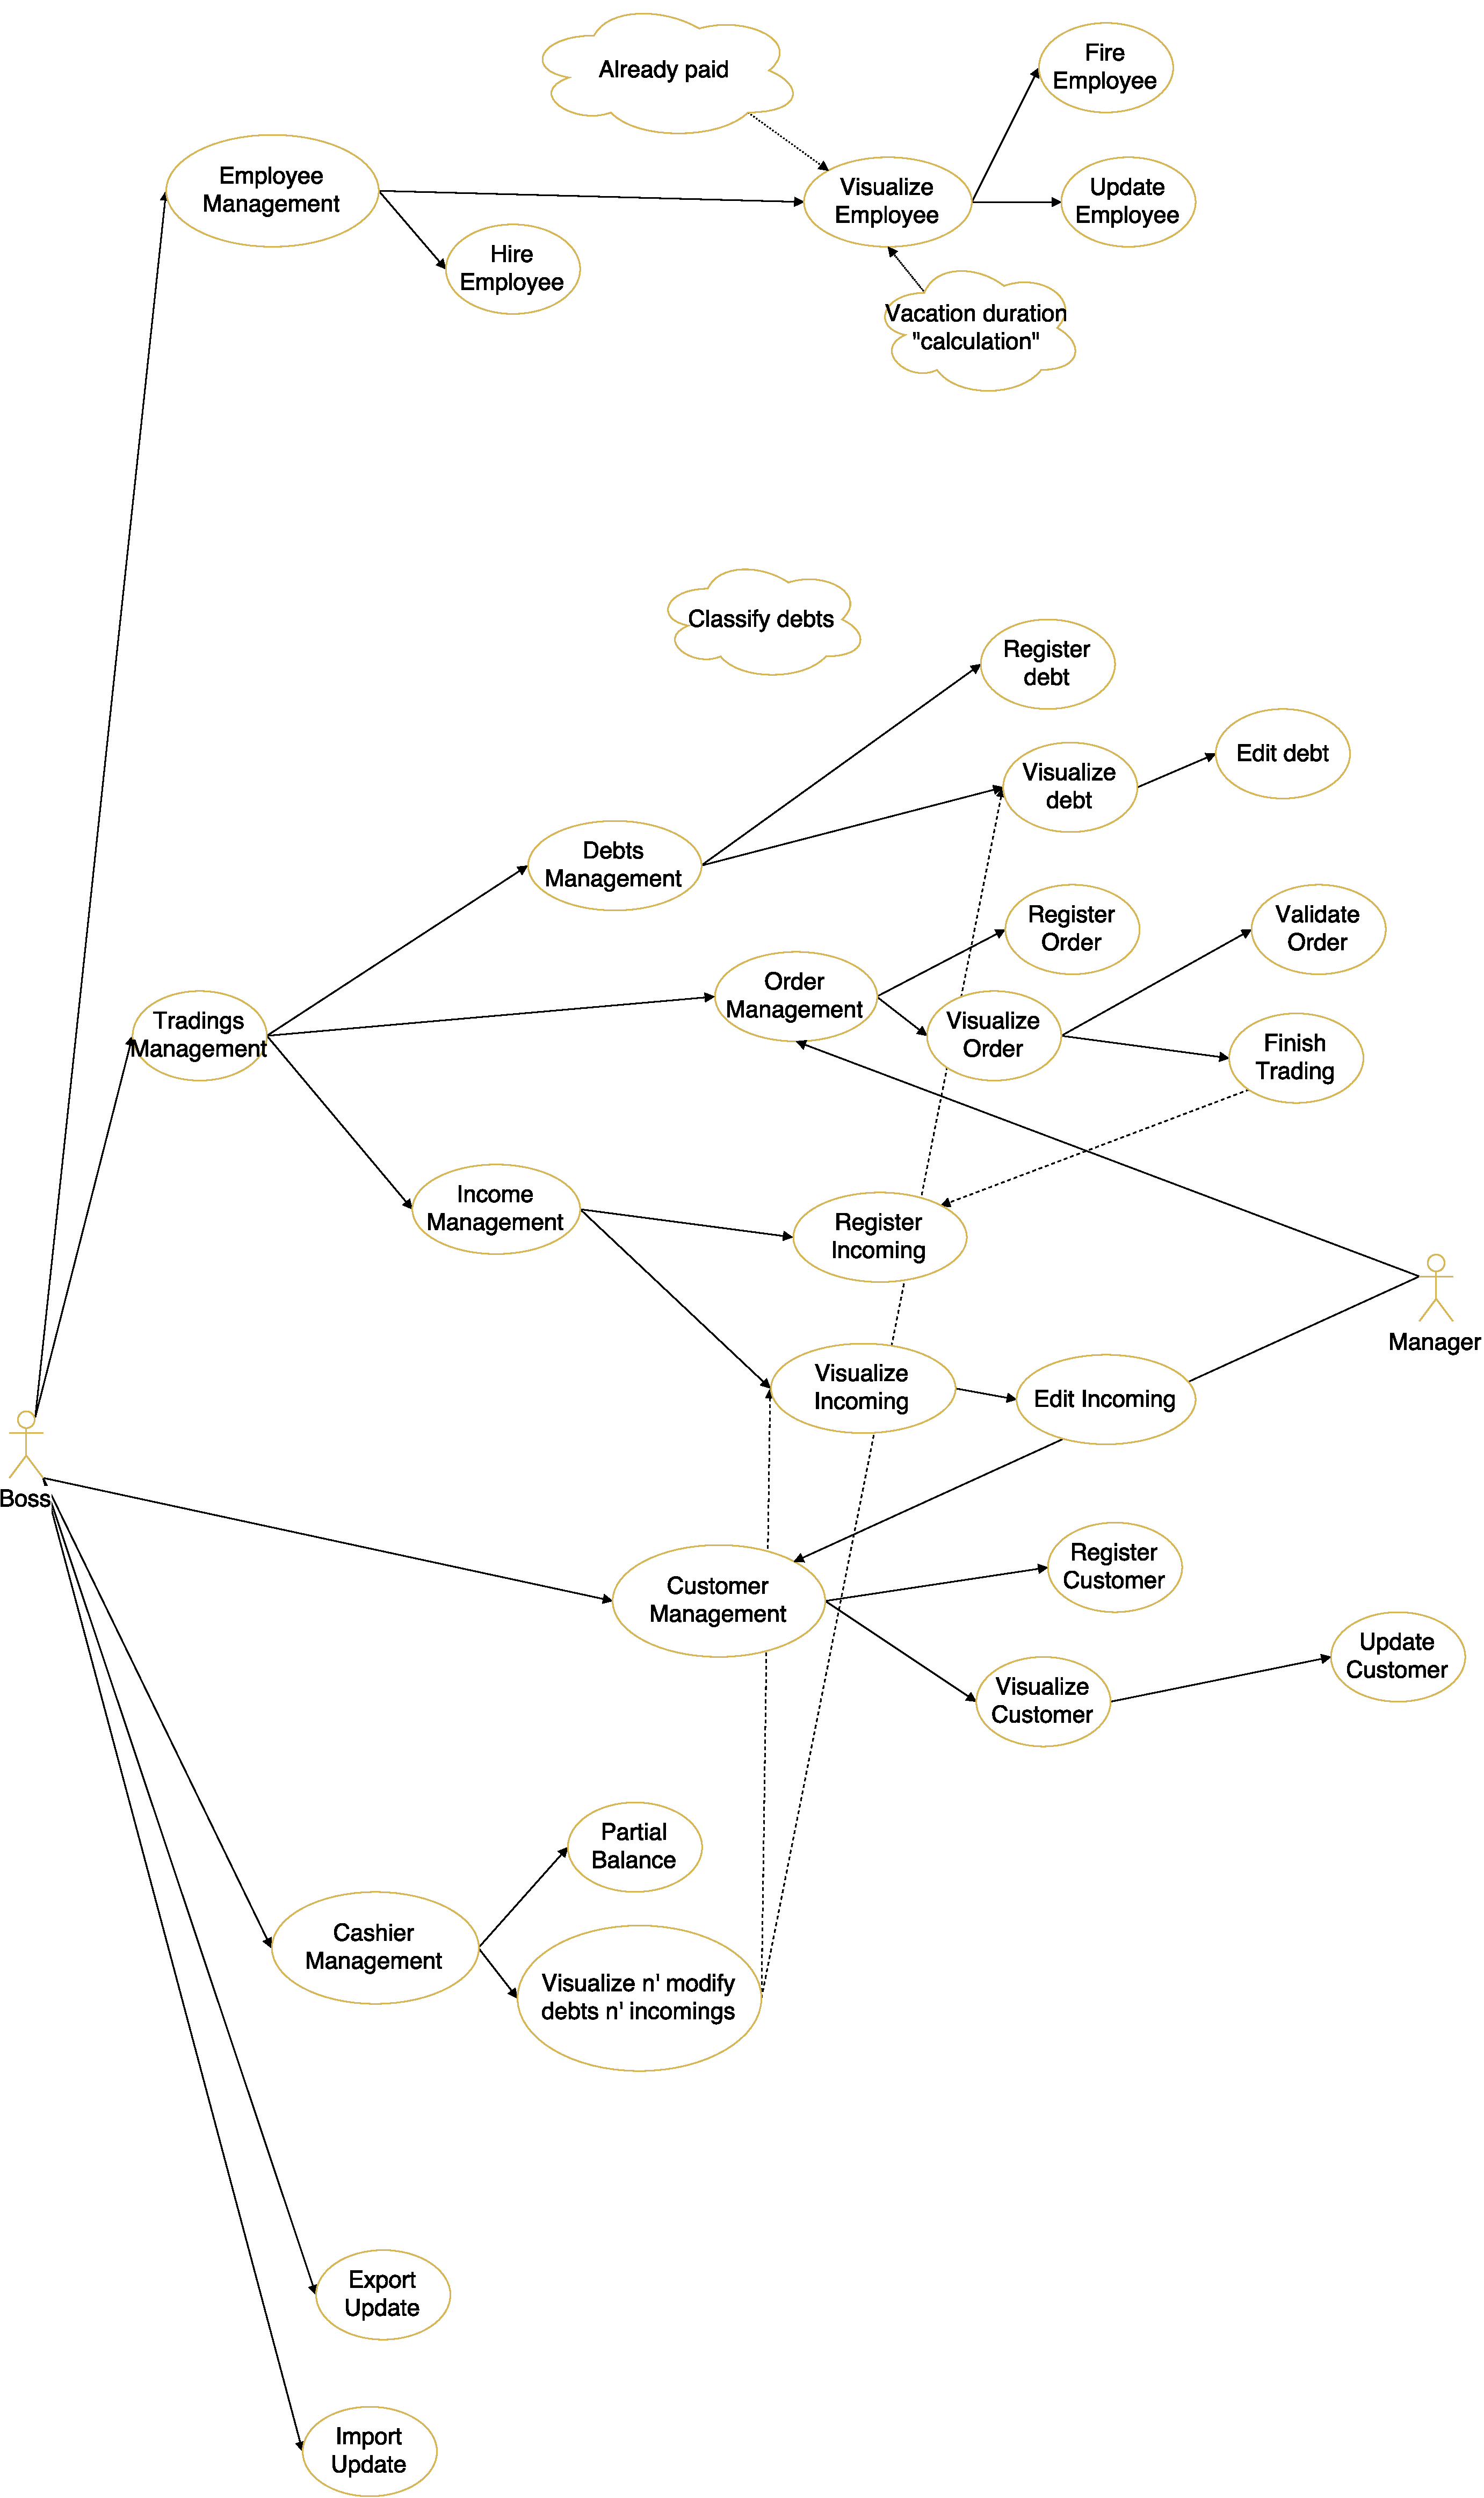
\includegraphics[width=\textwidth]{./UseCasesDiagramEnglish.pdf}
		\end{figure}
		\begin{figure}[H]
			\centering 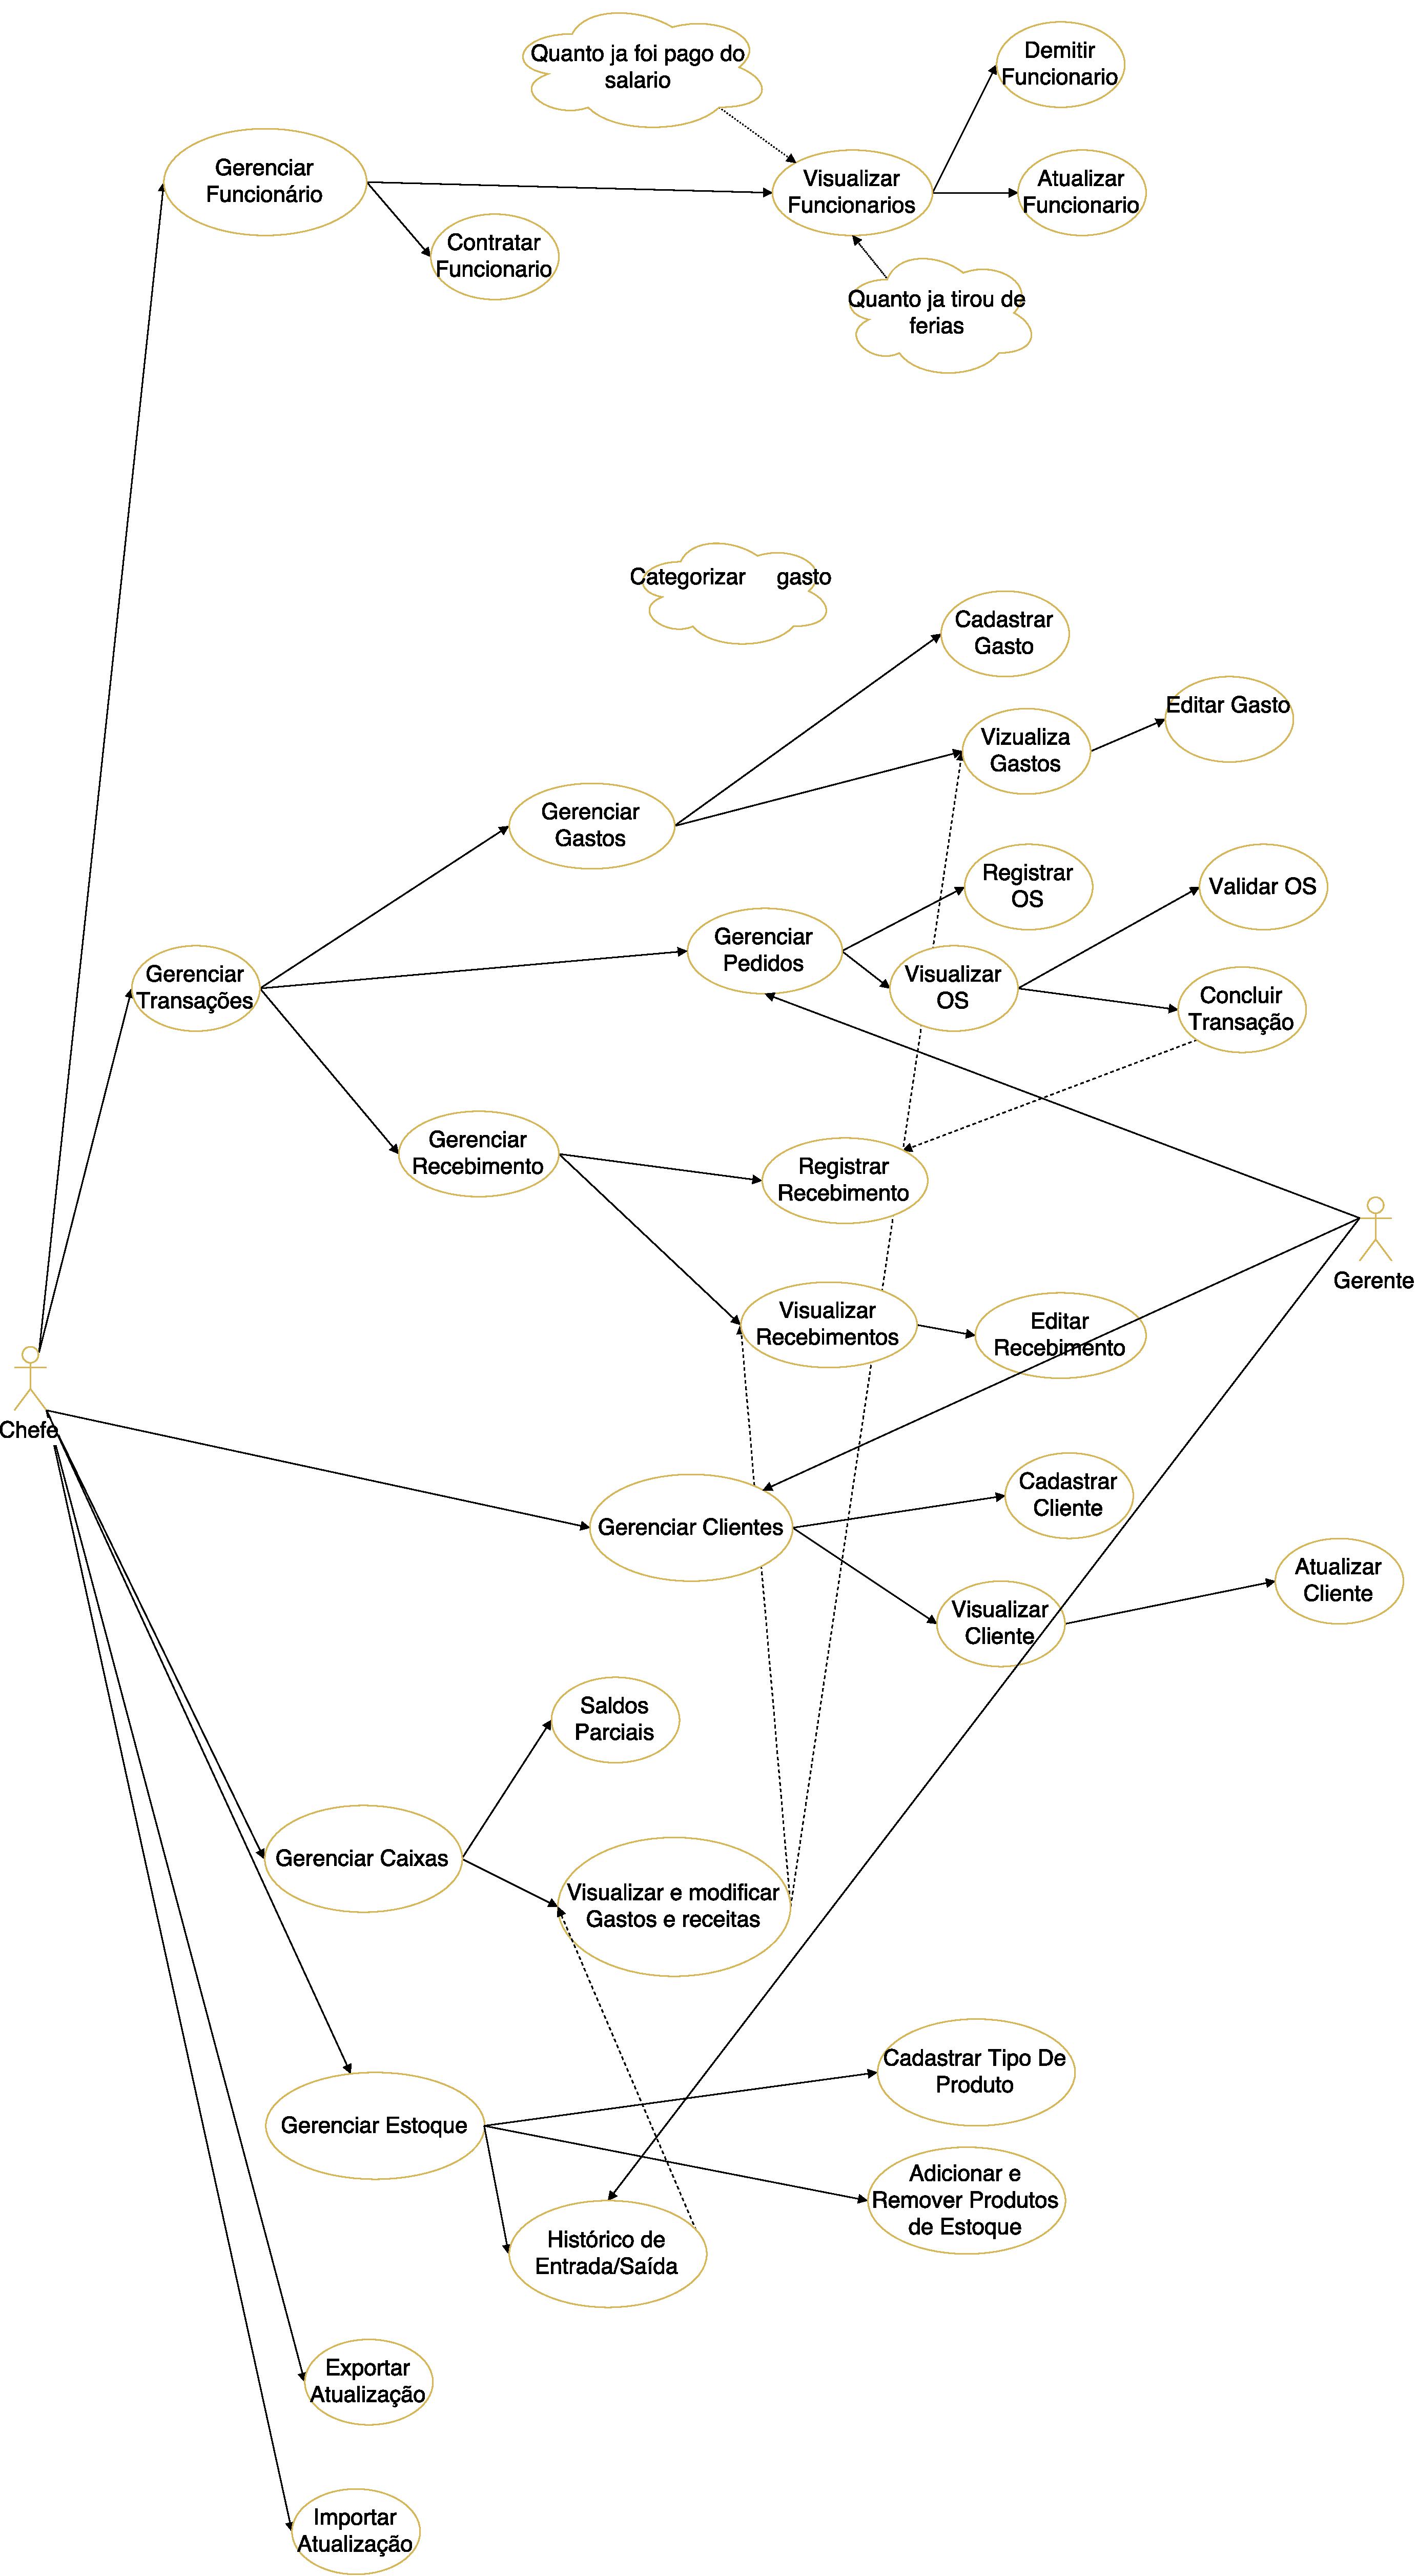
\includegraphics[width=\textwidth]{./DiagramaCasoDeUsoOficinaOld.pdf} 
		\end{figure}
		\begin{figure}[H]
			\centering 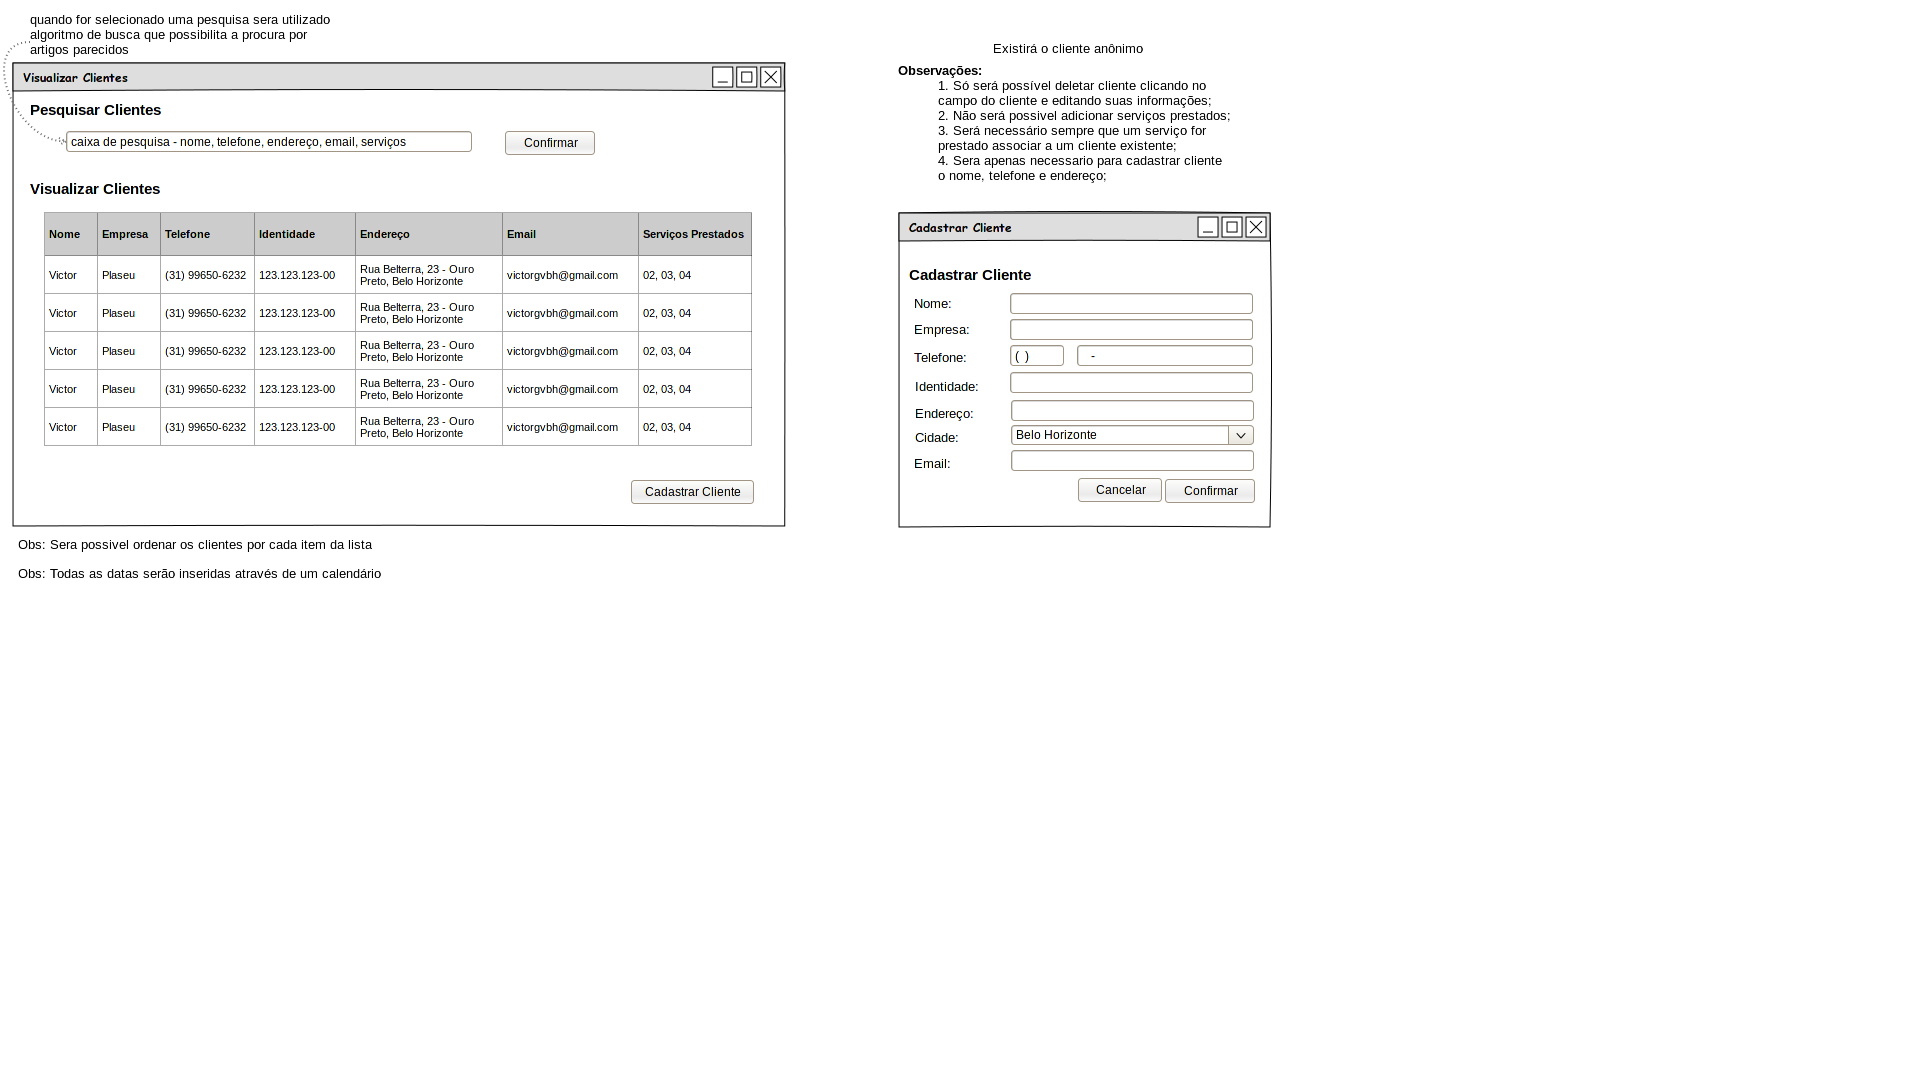
\includegraphics[width=\textwidth]{./Gerenciar Cliente.png}
		\end{figure}
		\begin{figure}[H]
			\centering 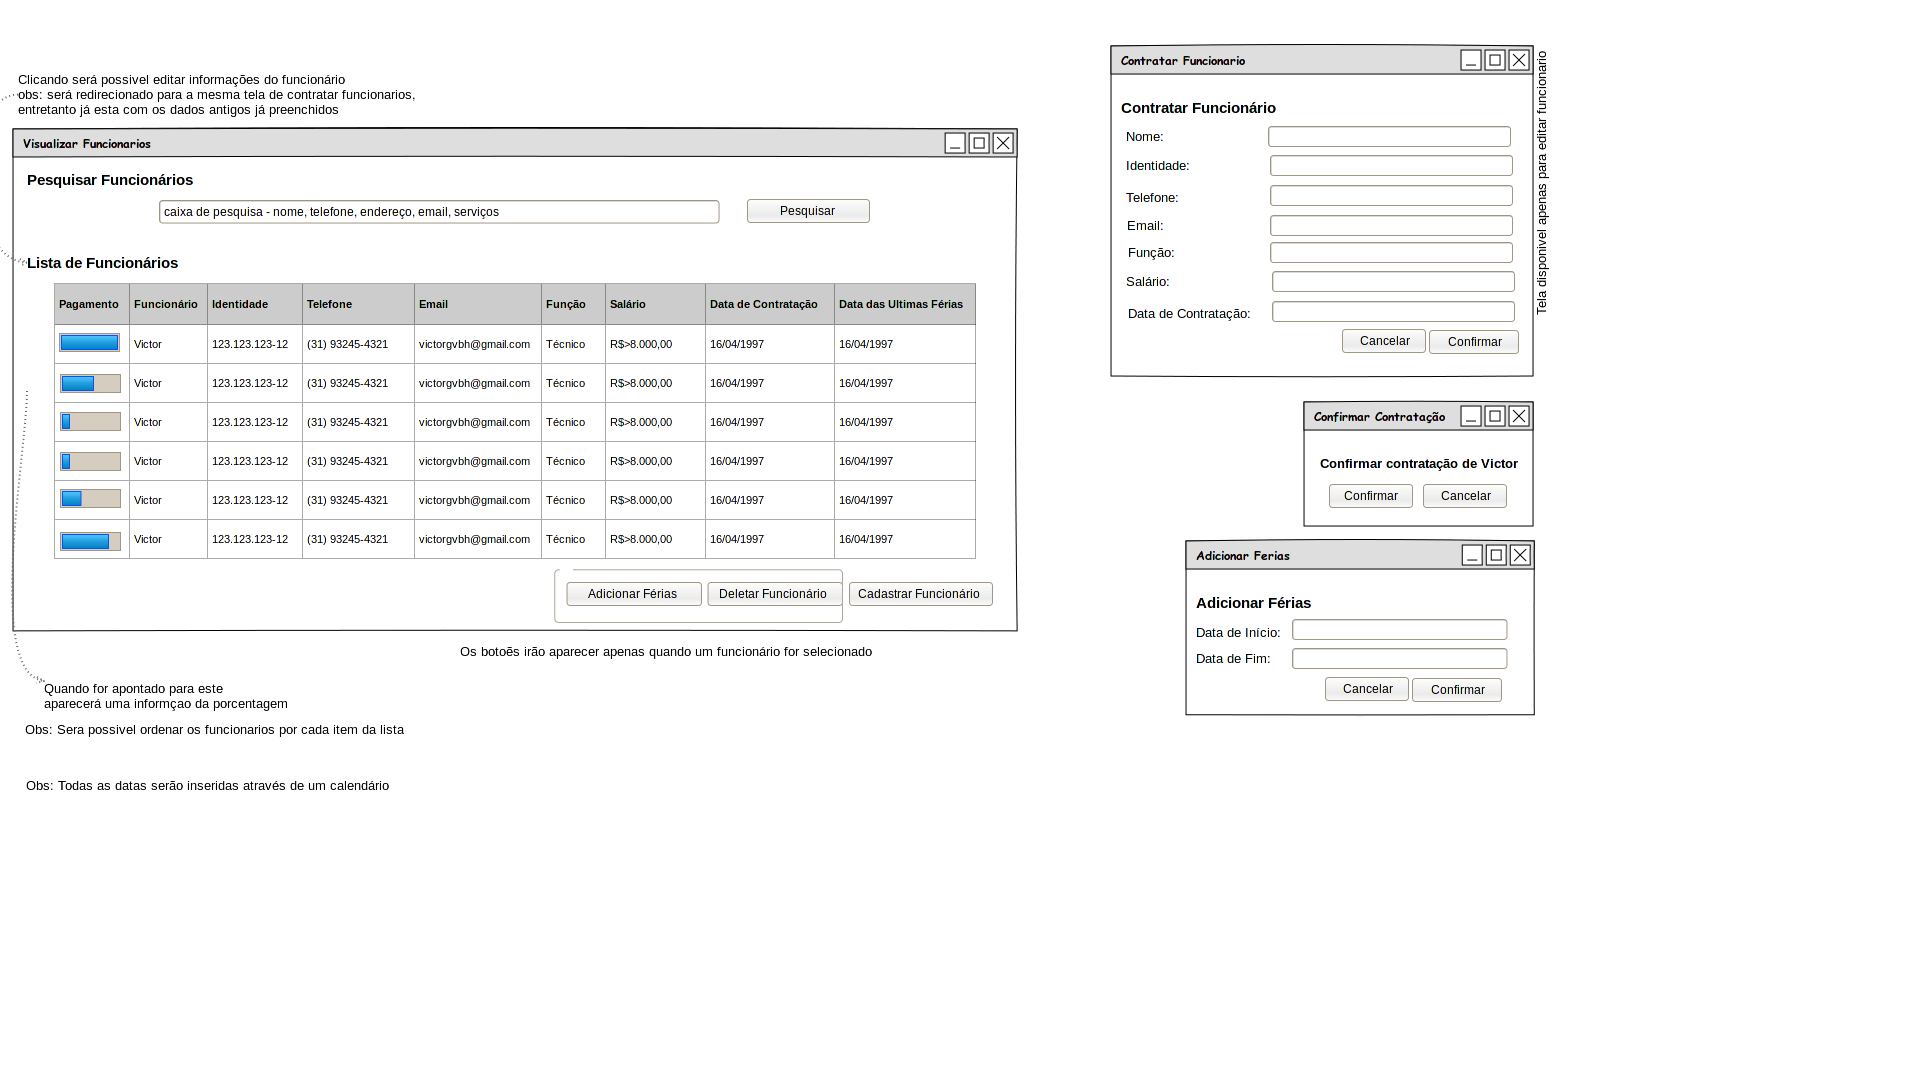
\includegraphics[width=\textwidth]{./Gerenciar Funcionario.png} 
		\end{figure}
		\begin{figure}[H]
			\centering 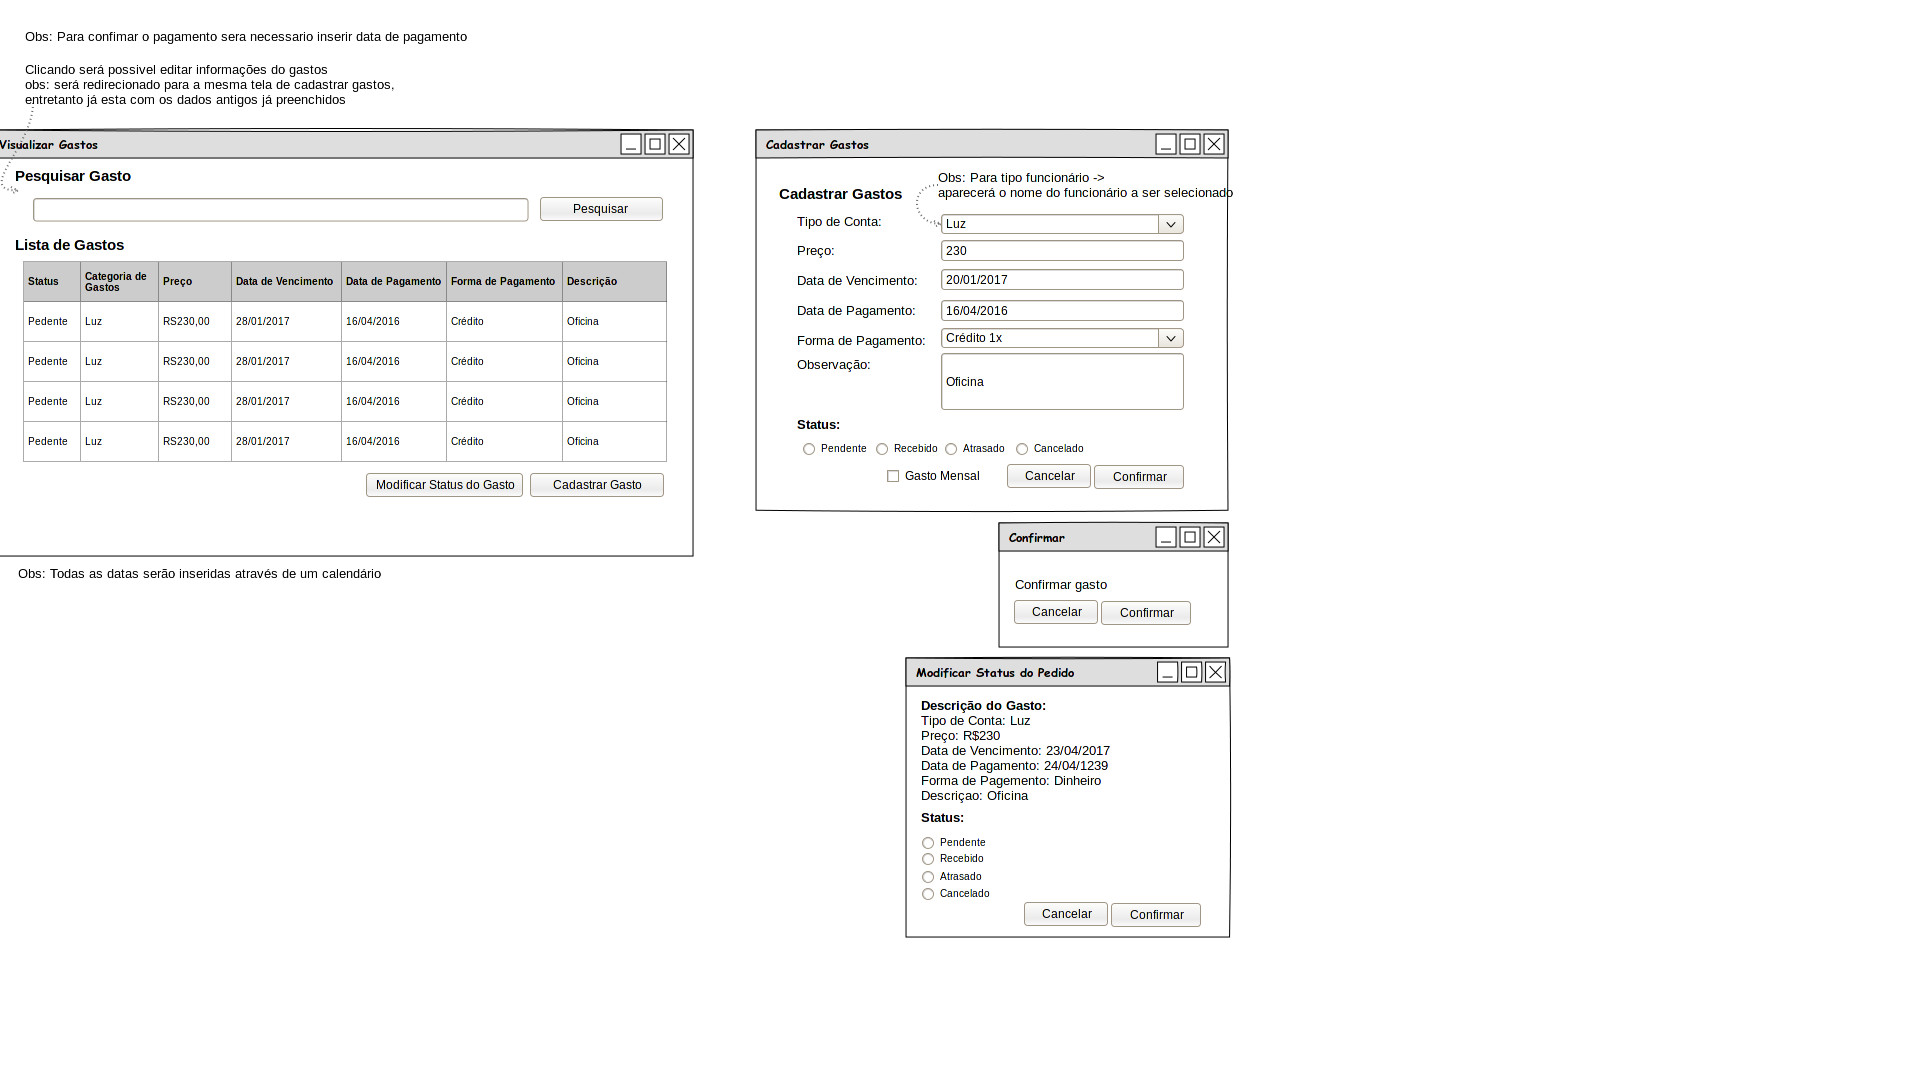
\includegraphics[width=\textwidth]{./Gerenciar Gastos.png} 
		\end{figure}
		\begin{figure}[H]
			\centering 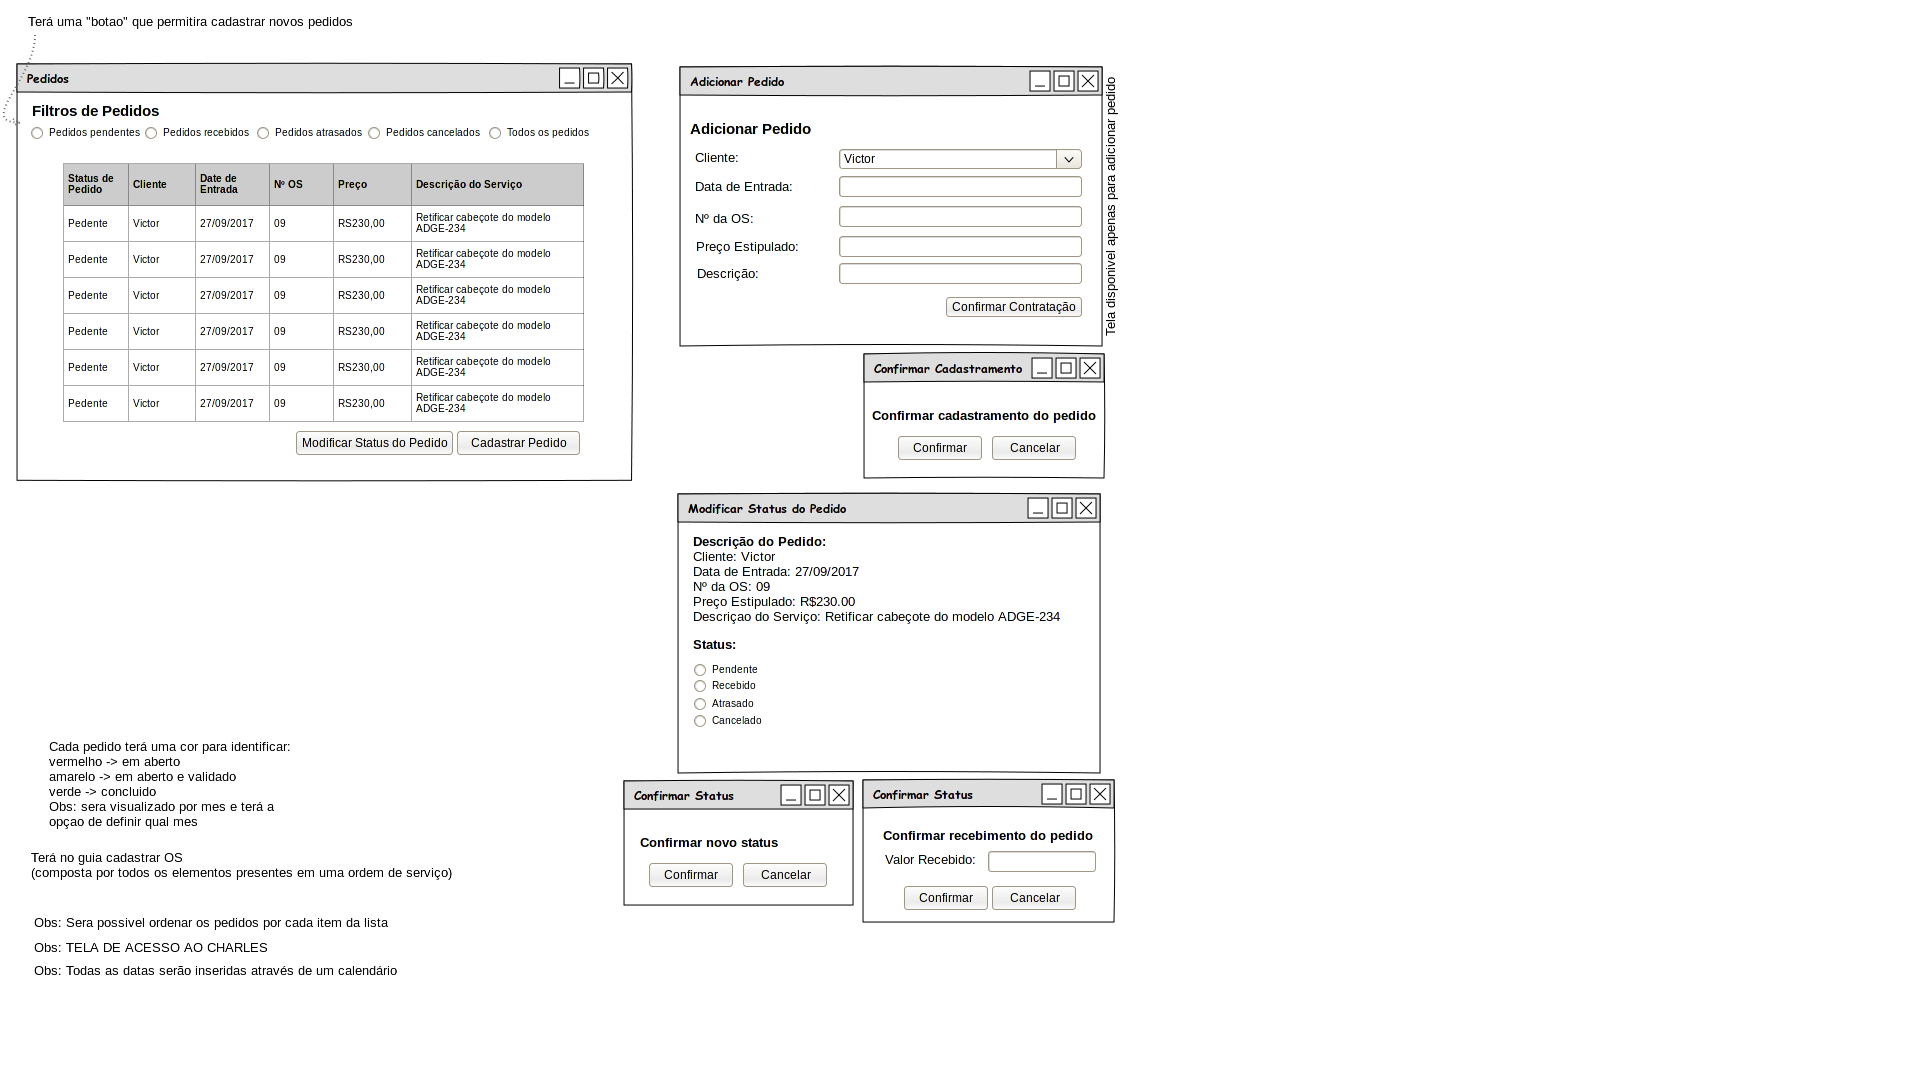
\includegraphics[width=\textwidth]{./Gerenciar Pedidos.png}
		\end{figure}
		\subsection{Licença} 
		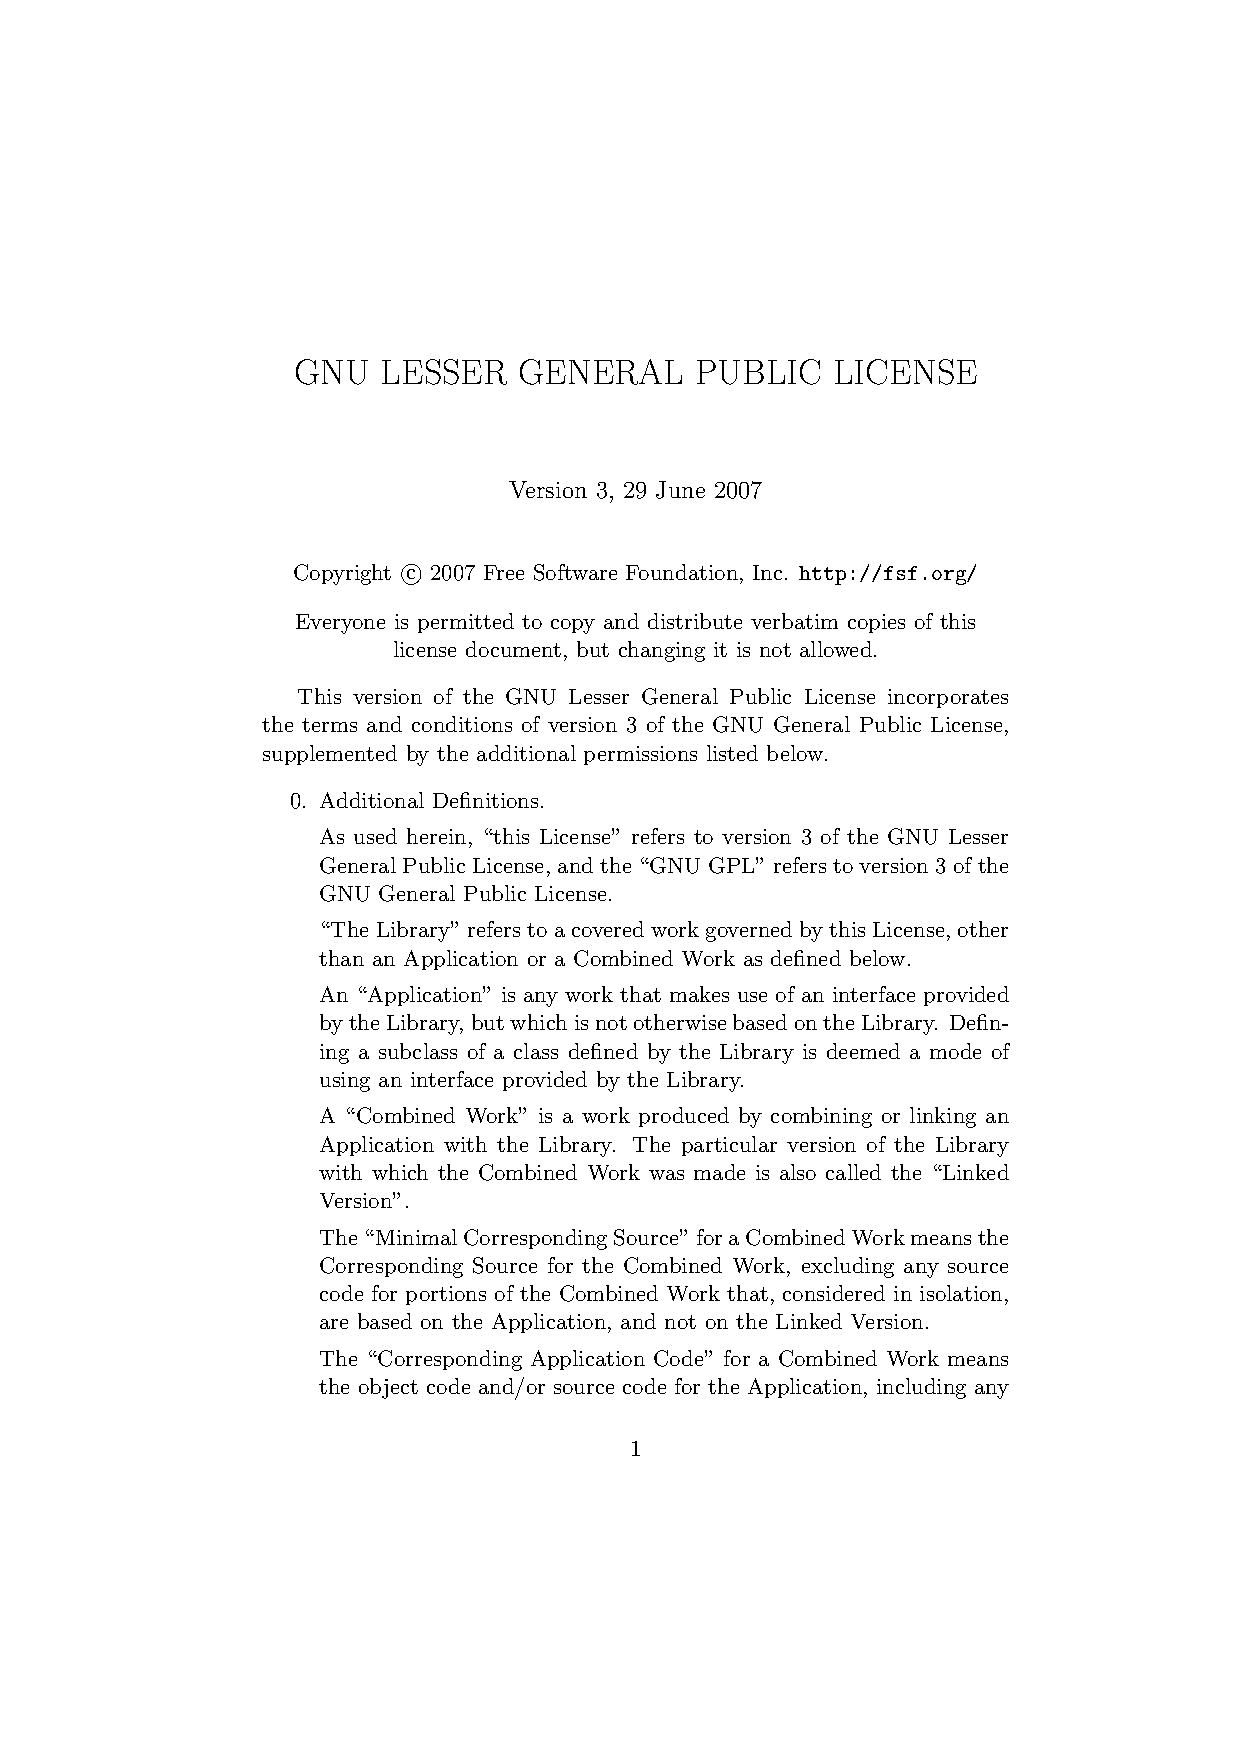
\includepdf[pages=-]{./lgpl-3-0.pdf}
		\subsection{Third-party source code used in our software}
		
		Nothing for now...
		
	\section{Tutorials and FAQ}
		\subsection{How to contribute to the project?}
		The contribution can be made by different ways:
		\begin{enumerate}
			\item Using and reporting bugs, or suggestion features to be incorporated into the program;
			\item ontributing informally: in case you already own any codes to be incorporated to the program, don't lose your time with formalities, send a pull request and one of our contributors shall study it and accept it if it meet our needs;
			\item Contributing formally: you can also become on of our formal colaborators! Just contact one of our organizers (Primary157, MessiahG), for more information on how to contact us, go to the "How to contact the organizers?" section.
		\end{enumerate}
		\subsection{How to contact the organizers?}
		The following lists points the contacts that we created exclusively to this project's audience:
		 \begin{enumerate}
		 	%\item Facebook:
		 	%\item Email: 
		 	\item IRC channel: \#businesssysman(freenode)
		 	%\item Twitter:
		 \end{enumerate}
		If you were not awnsered the way you expected or did not receive any awnsers, we also provide a list to contact each of us individually:
			\subsubsection{MessiahG}
			\begin{enumerate}
				\item Email: fadoa.glauss@gmail.com
				\item Github: fadoaglauss
			\end{enumerate}
			\subsubsection{Primary157}
			\begin{enumerate}
				\item Email: victorgvbh@gmail.com
				\item IRC: vgveloso(on freenode)
				\item Github: primary157
				\item Twitter: v\_gveloso
			\end{enumerate}
		\subsection{When will it be concluded?}
			Its too soon to think on a conclusion, but even when we meet the goals from the beginning of the project, we will still be active, developing more goals to better serve the business audience.
		\subsection{How to I install this software?}
			Unfortunately we still do not have an useable version of the program. But don't get your hopes down! We will keep you updater with what's happening in the project through Twitter and Facebook!
		\subsection{How do I use this software?}
			As soon as it reaches an useable version, you will find an user's manual here!
		\subsection{How to adopt this software to my company? Is there any technical support?}
			Unfortunately we can't confirm if we will ever get to offer technical support, but if that day ever comes, we will inform it through social media.
		\subsection{I have already downloaded and used it, but i found problems or thought of features that could be added. How to I get in contact?}
			Look in subsection "How to contribute to the project?" a few lines above!
		\subsection{What's the advantage of using this software?}
			You are contributing to a community of developers that look for making the implementation of company administration tech more accesible. You are also saving money, for this software is completely free.
		\subsection{Why C++, Qt and SQLite?}
			Our team pursuits the best possible results, even if development prices and costs are bigger. That being said, we chose C++ because its a high level, compilable language that empowers the developer.
			
			As we search for accessibility, there is nothing more interesting than being capable of running the software in any architecture or OS. For that, se chose Qt framework, which offers the forementioned characteristics while guaranteeing the same looks and functionalities in every system, this framework has a version with completely free license and promieses to deliver a nice looking responsive interface. 
	\section{References}
	%TODO Fazer a referencia
	\section{Special Thanks}
		Thanks to all who supported the creation and elaboration of this project, without your help it would now be preparing of its final rest in a dusty drawer. 
		
		For those who enter later in the project, we have not forgotten you. If your name isn't in the following list, make a pull request adding it.
		
		Developed by: Amaury, ZecaTapado, FadoaGlauss, Primary157, Astopho, Ramon, Daniel, Gabriel, Indiano, Lucas, Pedro, Zenon.
\end{document}
